\subsection{Training set generation}

To build SVM decision function representation from a range image the training set consisting of positive and negative example is necessary. In \cite{SVS2013} the authors work with shape images with white interior and black exterior. The positive examples are sampled from interior and the negative from exterior.

I introduce the range image interior as the part of space between the sensor and obstacles. Conversely, I call the part behind the obstacles exterior. I use the points of the range image as positive examples. The negative examples are obtained by the following algorithm:
\begin{enumerate}
\item
The normals are estimated at all the points of the range image and are oriented away from the sensor.
\item
Each positive example $p^+$ is shifted on the $w_{gap}$ distance in the normal direction to obtain a new negative example $p_{-}$, where $w_{gap}$ is the width of the gap, the algorithm's parameter. This value will be later referred to as \textit{local resolution} of the point cloud, since it is meant to approximate the distance beetween neighboring point of the range image in the vicinity of~$p^+$.
\end{enumerate}
The method is illustrated in the figure \ref{tset}. Its obvious disadvantage is its dependency on the normal estimation, which is known to be unstable. However, it is the only method I know which promises to generate the same negative examples for different sensor poses. In practice it works reasonably well (see figure XXX).
\begin{figure}
\centering
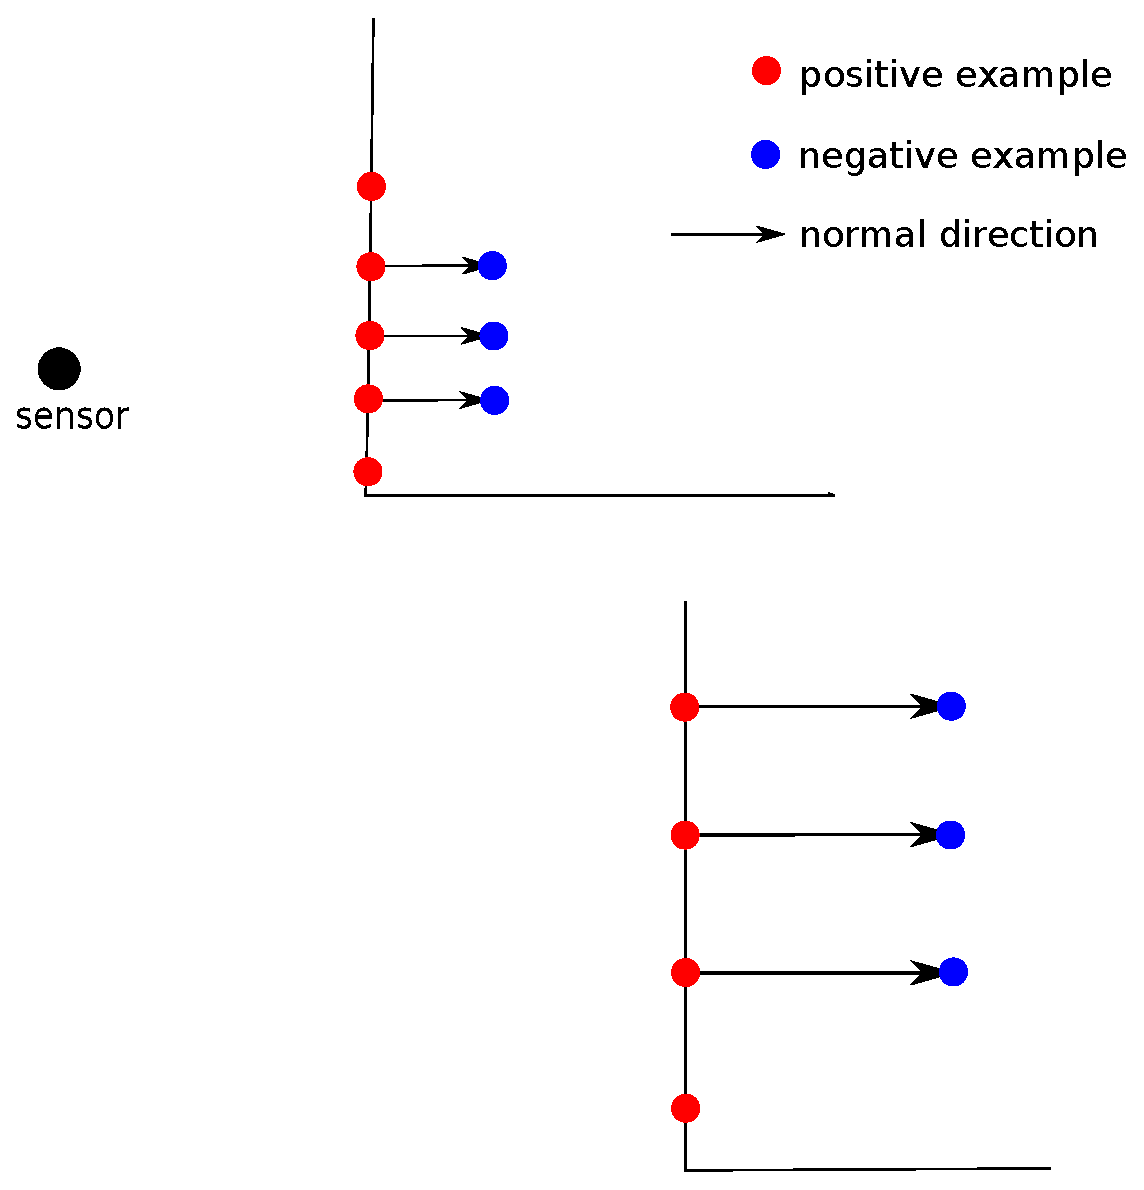
\includegraphics[scale=0.5]{training_set.eps}
\caption{Training set generation. The negative examples are shifted positive examples.}
\label{tset}
\end{figure}

\subsection{Extracting sparse Q structure from range image}
The points of range image are organized in $2D$ grid according to their spatial position. This property allows quick approximate search of all neighbors of given range image point $p$ within given radius~$R$. It is enough to consider the $r$ by $r$ square with the center in $p$, where $r=\Ceil{\frac{R}{\rho_{p}}}$, $\rho_{p}$ is average distance to the nearest neighbor for points in the vicinity of $p$. The points of the square can be than iterated with their distance to $p$ being checked to be less than $R$.

Using this approximate search algorithm the row of the $Q$ can be calculated on request. The modification is necessary to take care of negative examples: they are associated with the point of the range image they are obtained from. The calculated rows are stored in LRU cache, since despite its sparsity the full $Q$ matrix is too large to be stored in main memory. The cache faults are rare and do not impact the performance significantly (see corresponding section).

\subsection{Feature point search}
To find the feature points I start with the calculation of the gradient norm $||\nabla f||$ in all the range image points. The points in which the local maximum is reached are used as feature points. To check for local maximum in point $p$ I consider all the neighbors within the radius $R_{FP}$ and check that the gradient norm in all these points is less than in $p$.

\subsection{Parameters}
\label{sec:params}
The described feature extraction scheme has a lot of parameters and a systematic way for choosing them is required. This subsection describes one way do it: I start with a main parameter $\sigma$ called \textit{support size}. The support size specifies the level of details the algorithm should capture. As the final choice of feature points depends on the decision function it is natural to interpret $\sigma$ as the diameter of the ball which is large enough to discard all the support vectors that did not fall into it while computing the decision function in the ball center. The complementary parameters to $\sigma$ are two kernel thresholds $K_1$ and $K_2$. The $K_1$ is used to set the $\gamma$ parameter of the SVM in the following way:
\begin{equation}
\gamma = \frac{-4 \log (K_1)}{\sigma^2}
\end{equation}
to guarantee that within the support ball the kernel is always it least $K_1$. The second kernel threshold serves for making the $Q$ matrix sparse: all the elements less than $K_2$ are set to zero. I found it reasonable to fix $K_2=10^{-3}$ since it didn't hurt the quality of the $SVM$ model much and since the fine tuning of performance was not the aim. Another fixed parameter was $\epsilon_{KKT}=10^{-2}$: the threshold for $SVM$ convergence.

The choice of regularization parameter $C$ is non-trivial and is expected to be very data-source dependent. The evidence from the experiments says that in stable ares of the surfaces $\alpha_i$ stop their growth after some level, whereas in unstable regions they continue to steadily. This happens because of sensor noise and normal estimation errors on the object borders. Uncontrolled growth of $\alpha$ values can create gradient maximum regions caused by training set generation errors, which is highly undesirable. The figure \ref{fig:sv} illustrates the problem.
\begin{figure}
\centering
        \begin{subfigure}[b]{0.3\textwidth}
                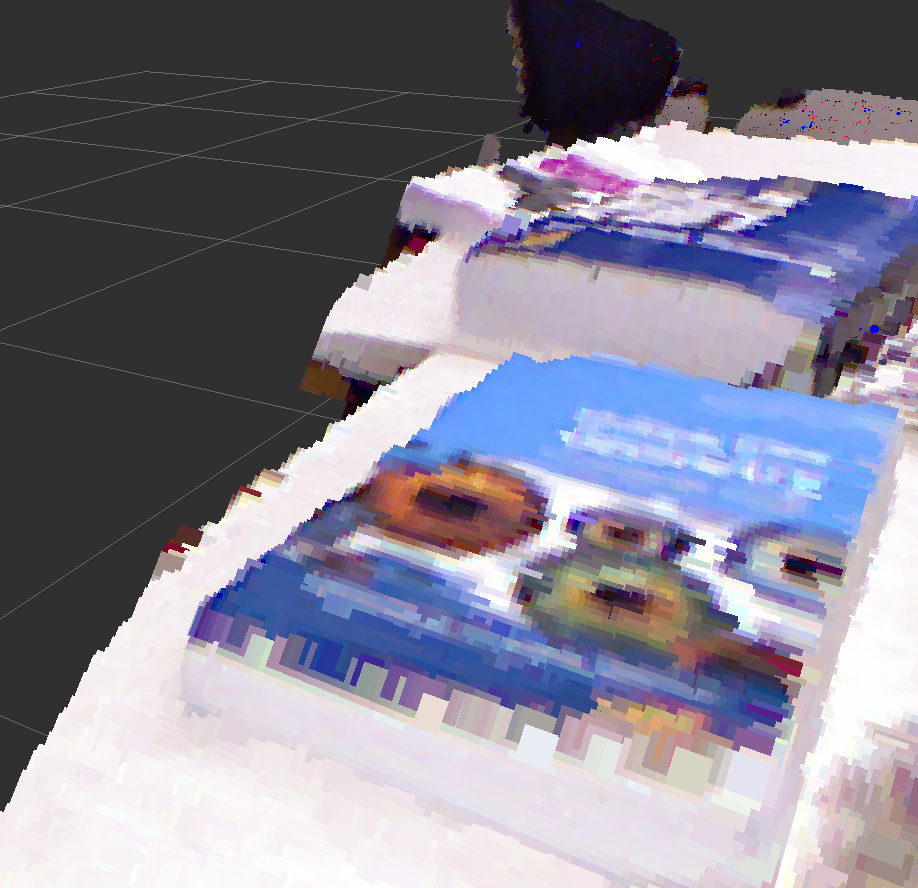
\includegraphics[width=\textwidth]{two_books.png}
                \caption{Sensor data}
                \label{fig:2books}
        \end{subfigure}%
        ~ %add desired spacing between images, e. g. ~, \quad, \qquad etc.
          %(or a blank line to force the subfigure onto a new line)
        \begin{subfigure}[b]{0.3\textwidth}
                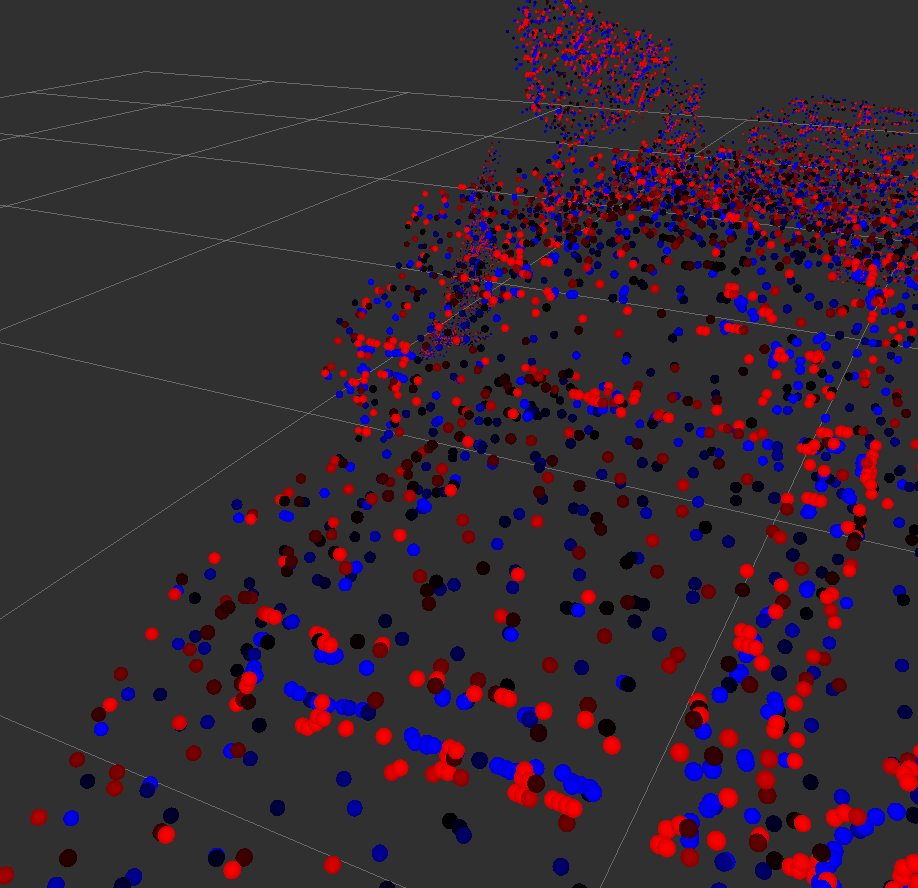
\includegraphics[width=\textwidth]{two_books_2.png}
                \caption{Support vectors, $C=2$}
                \label{fig:2books2}
        \end{subfigure}
        ~ %add desired spacing between images, e. g. ~, \quad, \qquad etc.
          %(or a blank line to force the subfigure onto a new line)
        \begin{subfigure}[b]{0.3\textwidth}
                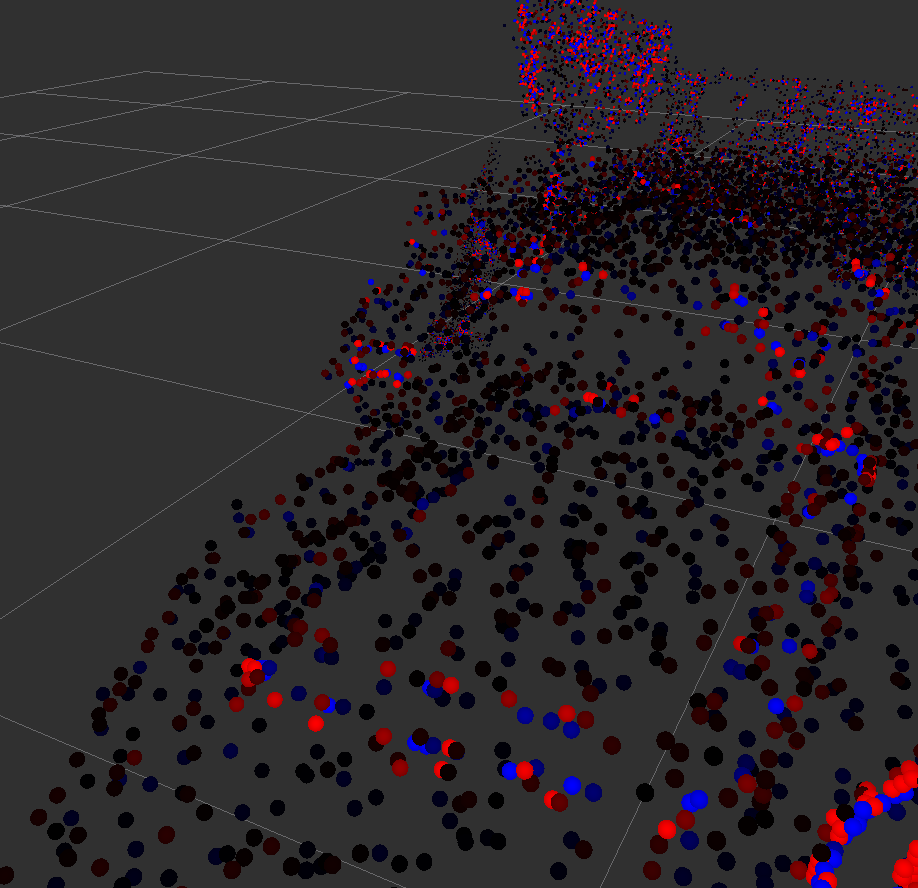
\includegraphics[width=\textwidth]{two_books_16.png}
                \caption{Support vectors, $C=16$}
                \label{fig:2books16}
        \end{subfigure}
\caption{The influence of the parameter $C$. The picture \ref{fig:2books} shows two books lying on a table. The other two pictures display support vectors learnt with different $C$ values. The red and blue components of sphere colors are $255 \frac{\alpha_i}{C}$ and $255\frac{C - \alpha_i}{C}$ correspondingly. One can see that in \ref{fig:2books16} a few noisy examples have much larger $\alpha_i$ values than all the others. They have high influence on gradient norm in their vicinity making feature extraction process less predictable and stable.} 
\label{fig:sv}
\end{figure}

Another non-trivial parameter is $w_{gap}$, the size of the gap between positive and negative examples. It is natural to set it proportional to sigma: $w_{gap} = \alpha_{gap} \sigma$, but it is not obvious what is the right value of $\alpha_{gap}$ coefficient. It is dangerous to set $\alpha_{gap}$ too large: the information contained in small- and middle-size changes of the shapes can be lost. Too small values of $\alpha_{gap}$ can lead to a uniform solution being optimal for SVM, when the positive and negative point clouds are almost inseparable. 

Summing up the parameter $\sigma$, $K_1$, $C$ and $\alpha_{gap}$ are subject to careful application-dependent choice. 
